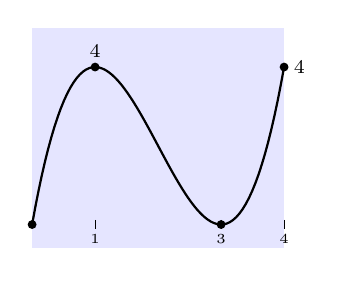
\begin{tikzpicture}[x=8mm,y=5mm]
\fill[blue!10] (0,-0.6) rectangle (4,5);
\ax{-0.6}{4.6}{-0.6}{5}
\draw[thick,domain=0:4,samples=80] plot (\x,{(\x)^3-6*(\x)^2+9*\x});
\draw (1,0.12)--(1,-0.12); \node[below] at (1,0){\tiny $1$};
\draw (3,0.12)--(3,-0.12); \node[below] at (3,0){\tiny $3$};
\draw (4,0.12)--(4,-0.12); \node[below] at (4,0){\tiny $4$};
\fill (1,4) circle (1.6pt);
\node[above] at (1,4){\scriptsize 4};
\fill (3,0) circle (1.6pt);
\fill (4,4) circle (1.6pt);
\node[right] at (4,4){\scriptsize 4};
\fill (0,0) circle (1.6pt);
\end{tikzpicture}